\documentclass[tikz,border=3pt]{standalone}
\usepackage[utf8]{inputenc}
\usepackage[T1]{fontenc}
\usepackage{lmodern}
\renewcommand{\familydefault}{\sfdefault}
\usepackage{sansmath}\sansmath
\usepackage{chemfig}
\usepackage{pgfplots}\pgfplotsset{compat=1.18,/pgf/number format/use comma,/pgf/number format/1000 sep={.}}
\usetikzlibrary{arrows.meta,calc,positioning,decorations.pathmorphing,patterns}
% paleta del sitio
\definecolor{nar}{HTML}{E8680C}\definecolor{narc}{HTML}{FFB35C}\definecolor{hielo}{HTML}{FFF3E8}
\definecolor{tinta}{HTML}{1D1D1F}\definecolor{gris}{HTML}{6E6E73}\definecolor{lila}{HTML}{7C5CF0}
\definecolor{azul}{HTML}{2F6FD6}\definecolor{menta}{HTML}{17A673}\definecolor{coral}{HTML}{E8342A}
\begin{document}
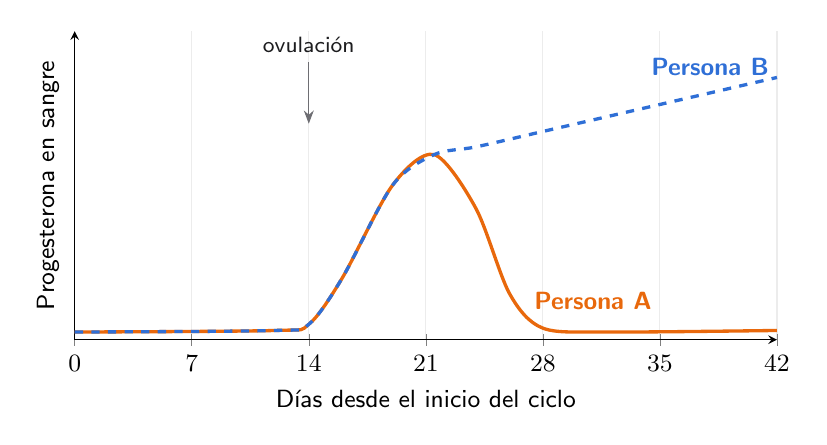
\begin{tikzpicture}[font=\small]
\begin{axis}[width=10.5cm,height=5.5cm,xmin=0,xmax=42,ymin=0,ymax=40,axis lines=left,ytick=\empty,xtick={0,7,...,42},
 xlabel={Días desde el inicio del ciclo},ylabel={Progesterona en sangre},grid=major,grid style={gray!15},clip=false]
\addplot[nar,very thick,smooth] coordinates {(0,1)(12,1.2)(14,2)(16,8)(19,20)(21.5,24)(24,17)(26,6)(28,1.5)(32,1)(42,1.2)};
\addplot[azul,very thick,smooth,dashed] coordinates {(0,1)(12,1.2)(14,2)(16,8)(19,20)(21.5,24)(24,25)(28,27)(32,29)(36,31)(42,34)};
\node[text=nar,font=\small\bfseries] at (axis cs:31,5) {Persona A};
\node[text=azul,font=\small\bfseries,anchor=south] at (axis cs:38,33) {Persona B};
\draw[gris,-{Stealth}] (axis cs:14,36) -- (axis cs:14,28) node[pos=0,anchor=south,text=tinta,font=\footnotesize] {ovulación};
\end{axis}
\end{tikzpicture}
\end{document}
